\chapter{Background} % nothing of mine

utrolig mye bra her: https://www.dei.unipd.it/\~emg/downloads/SIMPAR08-WorkshopProceedings/TeachingWithRobotics/karatrantou.pdf!! veldig mange bra kilder \hfill \\

og mange eksempler herfra: https://student.cs.uwaterloo.ca/~cs231/resources/pseudocode.pdf \hfill \\

This chapter will cover concepts that one should be familiar with in order to fully understand the rest of this thesis. We start by defining pseudocode to avoid confusion further down the line, as well as discussing transpiling, why Haskell is a good tool for the job, and how other transpilers work.

\section{Pseudocode}

Pseudocode is a technique for describing computer programs in a more abstract way than programming languages allow, ignoring specific syntax and keywords. This can make programs easier to understand for both non-programmers and programmers alike, when dealing with new situations \cite{LinfoAlgorithmsIntro2007}. \hfill \\

Since it does not follow any partifular syntax rules, pseudocode is also not executable. The whole point is that it is a way of \textit{presenting} code, rather than actually being code (rewrite needed) [kilde]. As such, pseudocode is an abstract concept, and can technically be anything, as long as it aims to aid others in understanding what a particular piece of code does [kilde]. \hfill \\

Usually, pseudocode is used at micro level, describing a \textit{part} of a problem, rather than the entire problem itself [kilde]. For example, when presenting a solution to a group of non-technical people, presenting pseudocode of an entire project might not always be insighful. However, presenting the programs core, or other pieces of code directly related to the programs core, might provide valuable insight to people who can come with suggestions for improvement, despite not being able to program it themselves.
\hfill \\

Now, since pseudocode has many faces, we must define what we percieve pseudocode to be in the context of this thesis, and what exactly we mean when we refer to ``pseudocode'' in later parts of the thesis. To avoid further confusion, we make a distinction between two particular types of pseudocode: text based and image based.

\subsection{Text based pseudocode}

The most common form of pseudocode is likely text based pseudocode, commonly found in text books on algorithms, published papers, as well as informal scribbling before attempting to solve a problem [kilder!]. It is also the form that most closely resembles source code, given that it usually includes line numbers and explains the steps in an imperative matter [kilde?]. \hfill \\

Since there is no proper set of rules commanding how text based pseudocode should look like, we are prone to viewing different variations of the same algorithms across different literatures. A frequently presented algorithm is Binary Search, which in the context of computer science is a search algorithm that finds the position of a target value within a sorted array \cite{BOOK:intro/Cormen/Leiserson}. \hfill \\

Here is how it is presented in The Design and Analysis of Computer Algorithms by Aho et. al in 1974 \cite[139]{BOOK:DesignAnalysis/Aho}:

\begin{lstlisting}
    procedure SEARCH(a, f, l):
    if f $>$ l then return "no"
    else
        if a = A[$\lfloor$(f + l)/2$\rfloor$] then return "yes"
        else
            if a < A[$\lfloor$(f + l)/2$\rfloor$] then
                return SEARCH(a, f, $\lfloor$(f + l)/2$\rfloor$ - 1)
            else return SEARCH(a, $\lfloor$(f + l)/2$\rfloor$ + 1, l)
\end{lstlisting}

Then, roughly 17 years later, Lewis et. al present it like this in Data Structures and Their Algorithms \cite[182]{BOOK:DSA/Lewis}:

\begin{lstlisting}[basicstyle=\small\ttfamily]
    function BinarySearchLookUp(key K, table T[0..n-1]): info
    {Return information stored with key K in T, or $\Lambda$ if K is not in T}
        Left $\gets$ 0
        Right $\gets$ n - 1
        repeat forever
            if Right < Left then
                return $\Lambda$
            else
                Middle $\gets$ $\lfloor$(Left + Right) / 2$\rfloor$
                if K = Key(T[Middle]) then return Info(T[Middle])
                else if K < Key(T[Middle]) then Right $\gets$ Middle - 1
                else Left $\gets$ Middle + 1
\end{lstlisting}

A desire for automatisation of text based pseudocode has been in the wind for a long time, with the intention of presenting ideas without having to worry about syntax of a particular programming language [kilde]. Text based pseudocode allows authors to draft ideas in an imperative way, just like we write recipes for baking bread and building legos. With pseudocode, the author is free to omit boilerplate code, include mathematical notation, include abstractions and revert to natural language where deemed appropriate \cite{BOOK:intro/Cormen/Leiserson}\cite{DBLP:conf/els/Nuallain15}. \hfill \\

As such, we can comfortably regard the succinctness of figure 2.1 displaying pseudocode, to figure 2.2 displaying an implementation of said pseudocode in a popular programming language \cite{LINCOPINIS2023}:

\begin{figure}[ht]
    \centering
    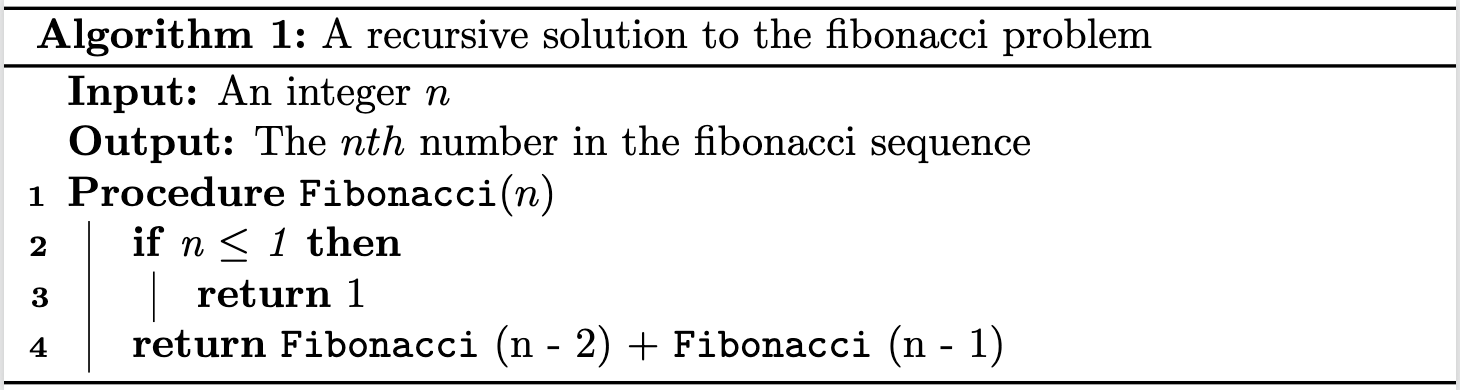
\includegraphics[scale=0.46]{assets/fibonacci_pseudo1.png}
    \caption{Text based pseudocode illustrating an algorithm to retrieve the nth number in a fibonacci sequence}
    \label{fig:fibseq1}
\end{figure}

\begin{figure}[ht]
    \centering
    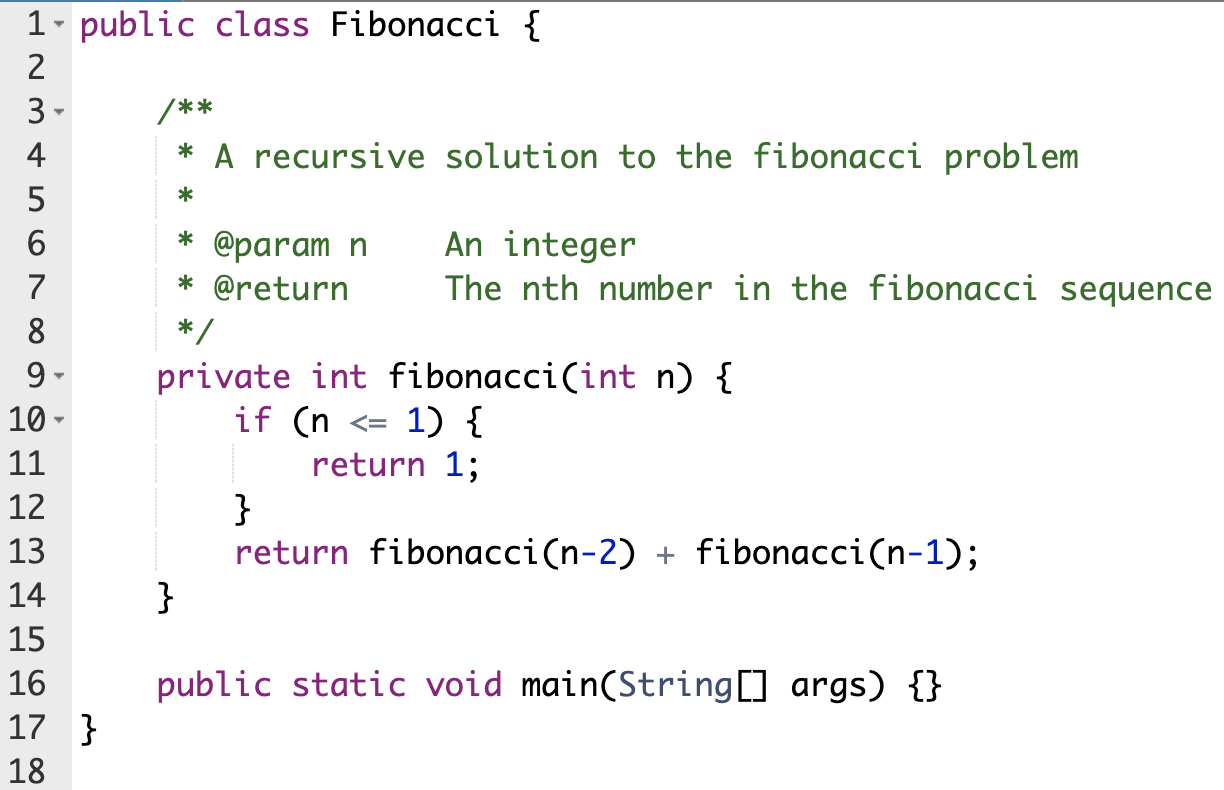
\includegraphics[scale=0.50]{assets/fibonacci_java.png}
    \caption{An algorithm written in the Java programming language, to retrieve the nth number in a fibonacci sequence. It follows the commenting guidlines JavaDoc\footnotemark.}
    \label{fig:fibjava}
\end{figure}
\footnotetext{https://docs.oracle.com/javase/8/docs/technotes/tools/windows/javadoc.html}

It is a useful tool when wishing to discuss unpolished ideas with friends and colleagues, but as mentioned, it has a rich history of being applied in university curriculums too [kilde]. When learning algorithms, datastructures, or programming concepts in general, the concepts tend to be more important than the specific implementation details in the author’s programming language of choice [kilde]. Thus, it can be advantageous for students to learn with pseudocode rather than source code, which could be a reason why there have been multiple attempts at translating source code to pseudocode in the past \cite{PSEU:/Kreher/Stinson}\cite{DBLP:conf/kbse/OdaFNHSTN15}\cite{DBLP:conf/aswec/AlhefdhiDHG18}. \hfill \\

Impact of pseudocode: https://iopscience.iop.org/article/10.1088/1757-899X/835/1/012044/pdf

\subsection{Image based pseudocode}

Not all programming languages share the same execution flow. For istance, in VHDL all processes are executed simultaneously\footnote{https://www.people.vcu.edu/~rhklenke/tutorials/vhdl/modules/m12\_23/sld008.htm}, whilst in Maude rules are applied in an arbitrary order [kilde]. Some, on the other hand, like Python, will execute their programs line for line. This means that we can follow the execution flow simply by looking at the order functions are called and the order of statements within those functions. \hfill \\

This way of executing a program opens up for the possibility of flowcharts, which still includes text, but also complements it with boxes, arrows and perhaps pretty colours. When code stretches over enough lines, it all starts looking similar and confusing [kilde]. Flowcharts, on the other hand, does a good job of isolating each statement, and potentially gives more of a birds eye view perspective of the code [kilde?]. \hfill \\

Throughout the remainder of this thesis, when we talk about ``image based pseudocode'', we are referring to flowcharts. The title does not technically need to belong to flowcharts, but it is the one we will concentrate on. \hfill \\

There have also been multiple attempts at creating flowchart editors, most notably by kilde1 et. al and kilde2 et. al [k1][k2]. This allows authors to visualise their ideas, rather than keeping it all text based. Benefits of learning with help from visual aid is well documented, e.g. when it comes to language learning and mathematics[kilde1][kilde2, kjøre noe roger antonen også eller? Sykt mange bra bilder i boka hans]. It seems a stretch to believe that students could not benefit from learning with images also when it comes to algorithms and programming concepts. \hfill \\

- figur(er)? \\

Given the imperative nature of flowcharts, the way they walk through problems step-by-step, it should not be impossible to convert image based psueodcode back to text based pseudocode. In fact, this has been attempted by kilde et. al, with positive results [kilde]. This gives even more ground to perceive flowcharts as an image based form of pseudocode. \hfill \\

- Vis bilde av ‘generating code FROM flowcharts' \\

Bra språk for å snakke om flowcharts: https://www.researchgate.net/publication/234805404\_Flowchart\_techniques\_for\_structured\_programming \\

Flowchart editor: https://www.researchgate.net/publication/234809385\_RAPTOR\_introducing\_programming\_to\_non-majors\_with\_flowcharts \\

Flowchart editor I think: https://ieeexplore.ieee.org/stamp/stamp.jsp?arnumber=4141379\&casa\_token=GEeSdBwgDfQAAAAA:6BaytVq0aANwj59lq2bHpcyMhV0enyZpOCuz93kEV\_tMaiQPHVY1OpwXO\_Gg1oDtxoKmfvXad4s \\

Generating code FROM flowcharts: https://www.scirp.org/html/7515.html \\

Impact of flowcharts: https://iopscience.iop.org/article/10.1088/1757-899X/835/1/012044/pdf

\section{Transpiling}
We have a program, we transform that into an intermediate representation, and from that intermediate representation we can get an entirely new representation. \hfill \\

An alternative to transpiling is the well-known phenomenon of \textit{compiling}. The difference is that we do not stay on the same abstraction level, but rather we make it much more specific. An example of this is compiling a Java file to bytecode. To humans, the bytecode reads like the most foreign language, though the JVM understands it perfectly, and is able to execute it. \hfill \\

\subsection{Generators}
One technique of utilising parsers and writers is to apply generators. A generator is basically a stand-alone parser or writer. A parser generator, in the context of Psnodig, would translate an example program to an AST, whilst a writer generator would translate an AST to a program. \hfill \\

An example of this is the programming language Derw\footnote{https://github.com/eeue56/derw}, an ML language mainly inspired by Elm. By utilising generators, it has multiple writers, among others bytecode, JavaScript, and even English. \hfill \\

Another example is Pandoc\footnote{https://github.com/jgm/pandoc}, which works with markdown languages. It has a ``core language'' which all parsers and writers must oblige to, and looks like this 

\begin{verbatim}
    Plain [Inline]
    Para [Inline]
    LineBlock [[Inline]]
    CodeBlock Attr String
    RawBlock Format String
    BlockQuote [Block]
    OrderedList ListAttributes [[Block]]
    BulletList [[Block]]
    DefinitionList [([Inline], [[Block]])]
    Header Int Attr [Inline]
    HorizontalRule
    Table [Inline] [Alignment] [Double] [TableCell] [[TableCell]]
    Div Attr [Block]
    Null
\end{verbatim}

BTW!! PANDOC PAPER: https://www.tug.org/TUGboat/tb35-1/tb109dominici.pdf \hfill \\

Every inputlanguage must be able to parse to (at least) these data types, and every writer must be able to work with these data types. \hfill \\

- Give example with e.g. HTML and MD for one of the data types?

\subsection{Haskell's strengths}
As previously mentioned, we opted for the Haskell programming language when implementing Psnodig. There are several reasons as to why, but the primary one is that it is widely perceived as a fitting tool when working with programming languages, and particularly when working with interpreters\footnote{https://github.com/Gabriella439/post-rfc/blob/main/sotu.md\#compilers}. At the end of the day, programming languages are just tools, and we believe this is the best one for this particular job. \hfill \\

With Haskell, it is straightforward to create your own \textbf{data types}, which are then used to model abstract syntax trees (ASTs). For instance, we can create our own calculator language in just a few lines of code:

\begin{verbatim}
    data Program = Program Expression

    data Expression =
          CompoundExpression Integer Operator Expression
        | IntExpression Integer

    data Operator =
          Plus
        | Minus
        | Times
        | Division
\end{verbatim}

From this, we can construct the following AST:

\begin{verbatim}
    Program (CompoundExpression 1 Plus
                (CompoundExpression 2 Minus
                    (IntExpression 3))
\end{verbatim}

As you can also see, we could create much bigger calculations than this, and if we wish to include extra operators, like for instance exponents in the future, we simply add a \texttt{| Exponent} to the Operator data type. \hfill \\

Another benefit of using Haskell, is that its strong type system opens for clean and efficient pattern matching. This is very useful, both when writing the interpreter, but also when adding new, potential readers. For example, if we wish to transpile the above AST to text, we could start with writing a function to convert the operators:

\begin{lstlisting}[caption={Haskell example to convert data type to string}, captionpos=b]
    f :: Operator -> String
    f (Operator Plus)     = " + "
    f (Operator Minus)    = " - "
    f (Operator Times)    = " / "
    f (Operator Division) = " * "
\end{lstlisting}

The function \textbf{f} takes something of type \textbf{Operator} as input, and returns something of type \textbf{String}. It will pattern match on the input, and return a correspondng value, making it bijective. We could add case of \texttt{f \_ = ""}, which would return the empty string for any other kind of operator, though this would be redundant as we have not defined any other type of operator anyway. \hfill \\

Lastly, we can utilise the QuickCheck\footnote{https://hackage.haskell.org/package/QuickCheck}, which is a testing library suited for automatic property-based testing in Haskell. With this we can prove different properties of our tool \cite{DBLP:conf/icfp/ClaessenH00}, and perhaps also of other (primarily) parsers and (maybe) writers, given that they have to pass through Haskell ADTs anyway.